\chapter{Arhitektura i dizajn sustava}
		
		%\textbf{\textit{dio 1. revizije}}\\

		%\textit{ Potrebno je opisati stil arhitekture te identificirati: podsustave, preslikavanje na radnu platformu, spremišta podataka, mrežne protokole, globalni upravljački tok i sklopovsko-programske zahtjeve. Po točkama razraditi i popratiti odgovarajućim skicama:}
	%\begin{itemize}
	%	\item 	\textit{izbor arhitekture temeljem principa oblikovanja pokazanih na predavanjima (objasniti zašto ste baš odabrali takvu arhitekturu)}
		%\item 	\textit{organizaciju sustava s najviše razine apstrakcije (npr. klijent-poslužitelj, baza podataka, datotečni sustav, grafičko sučelje)}
	%	\item 	\textit{organizaciju aplikacije (npr. slojevi frontend i backend, MVC arhitektura) }		
%	\end{itemize}

		Arhitektura našeg sustava dijeli se na tri podsustava: baza podataka, web aplikacija i web poslužitelj.
			
		\underbar{Web preglednik} program je koji služi kao posrednik između korisnika i web poslužitelja. Korisniku omogućuje pregled web-stranica te multimedijskih sadržaja vezanih uz njih. Svaka stranica pisana je u nekom kodu koji prosječnom korisniku ništa ne znači no kako je svaki internetski preglednik ujedno i prevoditelj, on prikazuje stranicu u obliku koja je svakome razumljiva. Na taj način korisnik šalje zahtjeve web poslužitelju.
		
		\underbar{Web poslužitelj} kao osnovnu zadaću ima ostvarivanje komunikacije između klijenta i aplikacije.  Ta komunikacija ostvarena je HTTP-om (engl. HyperText Transfer Protocol). Upravo je web poslužitelj temelj rada web aplikacije. On ju pokreće i prosljeđuje zahtjeve zaprimljene od web preglednika.
		
		\underbar{Web aplikacija} koju korisnik koristi obrađuje njegove zahtjeve. Ukoliko je potrebno za obradu zahtjeva, web aplikacija komunicira s poslužiteljem baze podataka koji joj dohvaća i prosljeđuje potrebne podatke. Potom web aplikacija vraća odgovor u obliku HTML dokumenta te web preglednik to prikazuje korisniku u odgovarajućem formatu.
		\begin{figure}
			\centering
			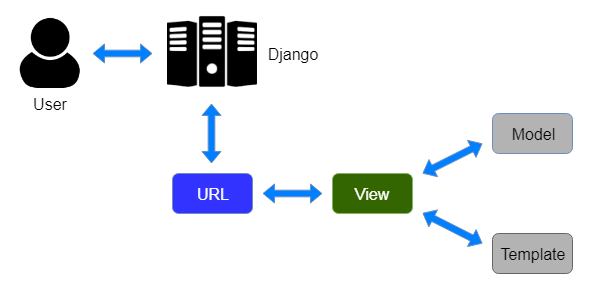
\includegraphics[width=0.7\linewidth]{../../MVT}
			\caption{MVT koncept}
			\label{fig:mvt}
		\end{figure}
		Za izradu naše web aplikacije odlučili smo se za programski jezik Python s njegovim radnim okvirom Django. Koristili smo Bootstrap, HTML, CSS i JavaScript za prikaz web-stranica. Baza podataka napisana je u PostgreSQL-u. Arhitektura sustava temeljit će se na MVT (engl. Model View Template) konceptu. S obzirom da je MVT koncept podržan od strane Djanga, na raspolaganju su nam gotovi predlošci te nam znatno olakšavaju razvoj web aplikacije.
	
		Zahvaljujući nezavisnosti razvoja pojedinih djelova aplikacije možemo jednostavnije ispitivati i razvijati sustav, kao i dodavati nova svojstva. Kao što se može pretpostaviti, MVT koncept sastoji se od triju komponenti. "Model" i "View" na strani su poslužitelja i nisu vidljivi korisniku, dok je "Template" vidljiv na korisnikovoj strani. "Model" središnja je komponenta sustava te pristupa bazi podataka. Pravilno formatira podatke dobivene od strane "View"-a te ih prosljeđuje bazi podataka i obrnuto. "View" prima podatke i zahtjeve kao što su "POST" i "GET" s klijentske strane. Također pravilno formatira primljene podatke te komunicira s druge dvije komponente MVT koncepta. "Template" služi za prikazivanje sadržaja na web-stranici. Sadrži statičke i dinamičke definicije prikaza sadržaja.
		
	
		
		

				
		\section{Baza podataka}
			
			\textbf{\textit{dio 1. revizije}}\\
			
		\textit{Potrebno je opisati koju vrstu i implementaciju baze podataka ste odabrali, glavne komponente od kojih se sastoji i slično.}
		
			\subsection{Opis tablica}
			

				\textit{Svaku tablicu je potrebno opisati po zadanom predlošku. Lijevo se nalazi točno ime varijable u bazi podataka, u sredini se nalazi tip podataka, a desno se nalazi opis varijable. Svjetlozelenom bojom označite primarni ključ. Svjetlo plavom označite strani ključ}
				
				\begin{longtabu} to \textwidth {|X[6, l]|X[6, l]|X[20, l]|}
					
					\hline \multicolumn{3}{|c|}{\textbf{korisnik - ime tablice}}	 \\[3pt] \hline
					\endfirsthead
					
					\hline \multicolumn{3}{|c|}{\textbf{korisnik - ime tablice}}	 \\[3pt] \hline
					\endhead
					
					\hline 
					\endlastfoot
					
					\cellcolor{LightGreen}IDKorisnik & INT	&  	Lorem ipsum dolor sit amet, consectetur adipiscing elit, sed do eiusmod tempor incididunt ut labore et dolore magna aliqua. Ut enim ad minim veniam 	\\ \hline
					korisnickoIme	& VARCHAR &   	\\ \hline 
					email & VARCHAR &   \\ \hline 
					ime & VARCHAR	&  		\\ \hline 
					\cellcolor{LightBlue} primjer	& VARCHAR &   	\\ \hline 
					
					
				\end{longtabu}
			
			
			\subsection{Dijagram baze podataka}
				\textit{ U ovom potpoglavlju potrebno je umetnuti dijagram baze podataka. Primarni i strani ključevi moraju biti označeni, a tablice povezane. Bazu podataka je potrebno normalizirati. Podsjetite se kolegija "Baze podataka".}
			
			\eject
			
			
		\section{Dijagram razreda}
		
			\textit{Potrebno je priložiti dijagram razreda s pripadajućim opisom. Zbog preglednosti je moguće dijagram razlomiti na više njih, ali moraju biti grupirani prema sličnim razinama apstrakcije i srodnim funkcionalnostima.}\\
			
			\textbf{\textit{dio 1. revizije}}\\
			
			\textit{Prilikom prve predaje projekta, potrebno je priložiti potpuno razrađen dijagram razreda vezan uz \textbf{generičku funkcionalnost} sustava. Ostale funkcionalnosti trebaju biti idejno razrađene u dijagramu sa sljedećim komponentama: nazivi razreda, nazivi metoda i vrste pristupa metodama (npr. javni, zaštićeni), nazivi atributa razreda, veze i odnosi između razreda.}\\
			
			\textbf{\textit{dio 2. revizije}}\\			
			
			\textit{Prilikom druge predaje projekta dijagram razreda i opisi moraju odgovarati stvarnom stanju implementacije}
			
			
			
			\eject
		
		\section{Dijagram stanja}
			
			
			\textbf{\textit{dio 2. revizije}}\\
			
			\textit{Potrebno je priložiti dijagram stanja i opisati ga. Dovoljan je jedan dijagram stanja koji prikazuje \textbf{značajan dio funkcionalnosti} sustava. Na primjer, stanja korisničkog sučelja i tijek korištenja neke ključne funkcionalnosti jesu značajan dio sustava, a registracija i prijava nisu. }
			
			
			\eject 
		
		\section{Dijagram aktivnosti}
			
			\textbf{\textit{dio 2. revizije}}\\
			
			 \textit{Potrebno je priložiti dijagram aktivnosti s pripadajućim opisom. Dijagram aktivnosti treba prikazivati značajan dio sustava.}
			
			\eject
		\section{Dijagram komponenti}
		
			\textbf{\textit{dio 2. revizije}}\\
		
			 \textit{Potrebno je priložiti dijagram komponenti s pripadajućim opisom. Dijagram komponenti treba prikazivati strukturu cijele aplikacije.}